\documentclass[9pt]{beamer}
\mode<presentation>

% Theme choice:
\usetheme{Madrid}%Darmstadt 

\usecolortheme[RGB={0,100,50}]{structure}
 \usefonttheme{structurebold} 
\setbeamercovered{invisible}
%\setbeamertemplate{navigation symbols}{}
\usepackage{dynblocks}
\usepackage{textpos}
\usepackage{amsfonts}
\usepackage{amsmath}
\usepackage{amssymb}
\usepackage{amsthm}

\newtheorem{teorema}{Teorema}\usepackage{mathtools}
\renewcommand{\proofname}{Prova}
\usepackage[portuguese]{babel}

\uselanguage{Portuguese}
\languagepath{Portuguese}

\deftranslation[to=Portuguese]{Theorem}{Teorema}
\deftranslation[to=Portuguese]{Lemma}{Lema}
\deftranslation[to=Portuguese]{Corollary}{Corolário}
\deftranslation[to=Portuguese]{Proof}{Prova}

\usepackage{dutchcal}
\usepackage{hyperref}
\usepackage[utf8]{inputenc}
\usepackage[T1]{fontenc}
\usepackage{amsthm}


\usepackage[affil-it]{authblk} 
\usepackage{etoolbox}
\usepackage{lmodern}

\makeatletter
\patchcmd{\@maketitle}{\LARGE \@title}{\fontsize{18}{19.2}\selectfont\@title}{}{}
\makeatother

\renewcommand\Authfont{\fontsize{12}{14.4}\selectfont}
\renewcommand\Affilfont{\fontsize{9}{10.8}\itshape}

% Title page details: 
\title[Presentation]{Programação Orientada a Objetos} %add title


\institute[UniRV]{\textbf{\large  \textcolor{structure}{\textbf{\large
Classes, objetos, atributos e métodos.
}} %add name 
% \hspace{0.5pt}
\\ \qquad
\\Professor: Me. Sergio Souza Novak 
\\Faculdade de Engenharia de Software}
} 
% \titlegraphic{\includegraphics[width=5cm]{msu.eps}}
\titlegraphic{
\includegraphics[width=5cm]{Universidade_de_Rio_Verde.jpg}}
\date{}

% Logo only on title page
%\logo{
\includegraphics[width=1cm,keepaspectratio]{Logo.png}}
\usepackage[pscoord]{eso-pic}


\begin{document}

% Title page frame
%\begin{frame}
    %\titlepage 
%\end{frame}
\frame[plain]{\titlepage}
%logo
\AddToShipoutPictureFG{
    \put(\LenToUnit{.92\paperwidth},
    \LenToUnit{.185\paperheight})
    {\vtop{{\null}
    \makebox{
\includegraphics[width=.8cm,keepaspectratio]{Universidade_de_Rio_Verde.jpg}}}}}


\begin{frame}{Sumário}
  \tableofcontents
\end{frame}
\section{Relembrando o paradigma Orientação a Objetos}



\begin{frame}{Paradigma de Orientação a Objetos}

\begin{block}{Definição}
O paradigma de \textbf{Orientação a Objetos (OO)} é um modelo de programação
baseado na organização do software em \textbf{objetos}, que representam
entidades do mundo real ou conceitos abstratos.

Cada objeto é composto por:
\begin{itemize}
    \item \textbf{Estado} (atributos)
    \item \textbf{Comportamento} (métodos)
\end{itemize}
\end{block}

\begin{block}{Conceitos Fundamentais}
\begin{itemize}
    \item \textbf{Classe}: molde ou modelo que define atributos e métodos.
    \item \textbf{Objeto}: instância concreta de uma classe.
    \item \textbf{Encapsulamento}: proteção e controle de acesso aos dados.
\end{itemize}
\end{block}

\begin{block}{Objetivo do Paradigma}
Promover:
\begin{itemize}
    \item Modularidade
    \item Reutilização de código
\end{itemize}
\end{block}

\end{frame}
\begin{frame}{Paradigma Orientado a Objetos}
O paradigma orientado a objetos (POO) organiza o software em  \textbf{classes}, que são moldes para os \textbf{objetos}, entidades do mundo real.\begin{figure}
\centering
\begin{minipage}{0.45\textwidth}
  \centering
  
\includegraphics[width=\textwidth]{classe_ovo.jpeg}
  \caption{Classe}
\end{minipage}
\hfill
\begin{minipage}{0.45\textwidth}
  \centering
  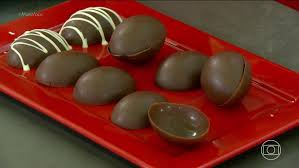
\includegraphics[width=\textwidth]{objeto_ovo.jpeg}
  \caption{Objeto}
\end{minipage}
\end{figure}


\end{frame}
\section{Classes}

\begin{frame}{Classe em Orientação a Objetos}

\begin{figure}
    \centering
    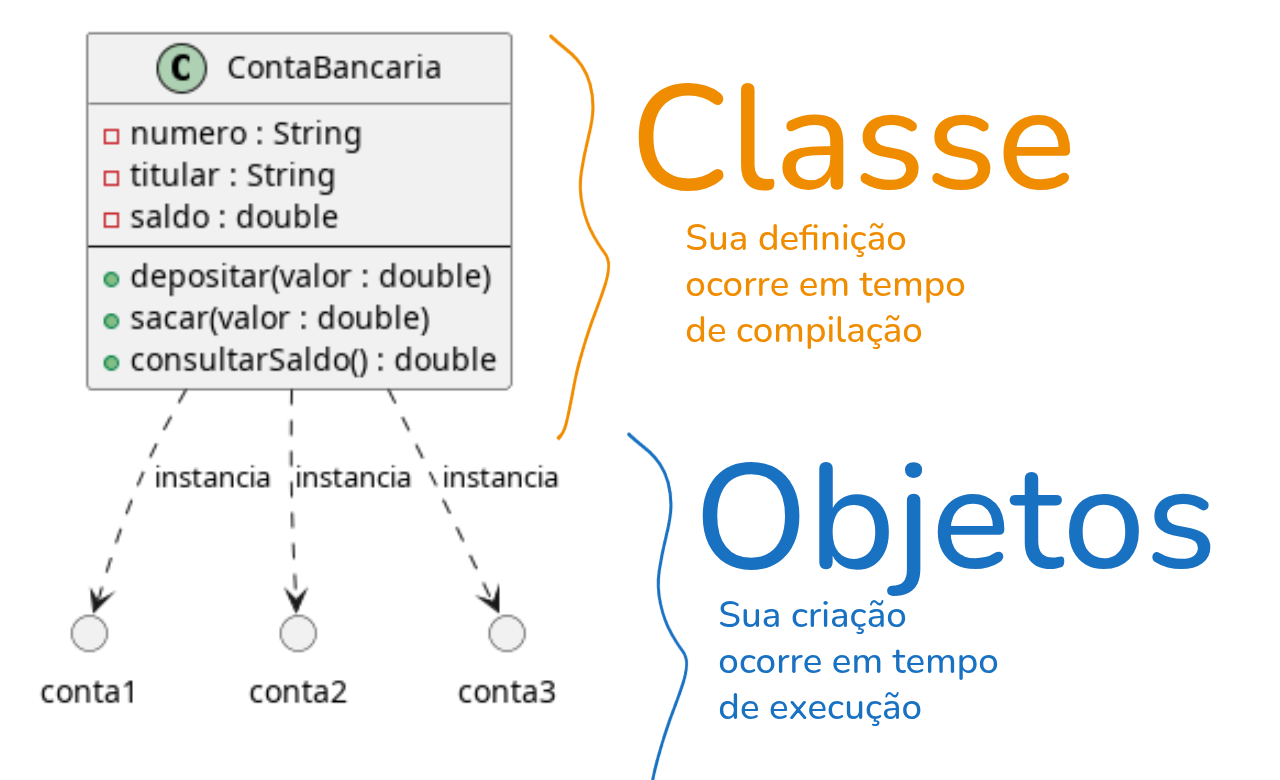
\includegraphics[width=\linewidth]{classeseobjetos.png}
    % \caption{Representação ilustrativa de uma classe em JAVA}
\end{figure}
\end{frame} 
\begin{frame}{Classe em Orientação a Objetos}

\begin{block}{Definição Formal}
Uma \textbf{classe} é uma estrutura abstrata que define um tipo de objeto.
Ela especifica:
\begin{itemize}
    \item O conjunto de \textbf{atributos} (estado)
    \item O conjunto de \textbf{métodos} (comportamento)
\end{itemize}
A classe funciona como um \textit{molde} para a criação de objetos.
\end{block}

\begin{figure}
    \centering
    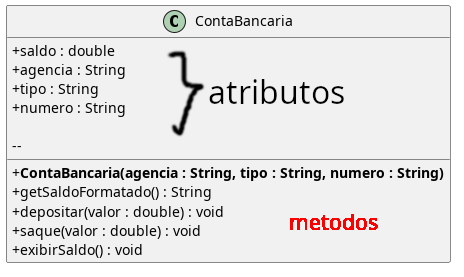
\includegraphics[width=0.7\linewidth]{ContaBancariaUml.png}
    \caption{Representação ilustrativa de uma classe em UML}
\end{figure}
 
% \begin{block}{Estrutura Conceitual}
% De forma geral, uma classe pode ser representada como:
% \[
% \text{Classe} = \{ \text{Atributos}, \text{Métodos} \}
% \]

% Onde:
% \begin{itemize}
%     \item \textbf{Atributos}: variáveis que armazenam o estado do objeto.
%     \item \textbf{Métodos}: funções que definem as operações permitidas.
% \end{itemize}
% \end{block}
\end{frame}

\begin{frame}{Classe em Orientação a Objetos}

\begin{figure}
    \centering
    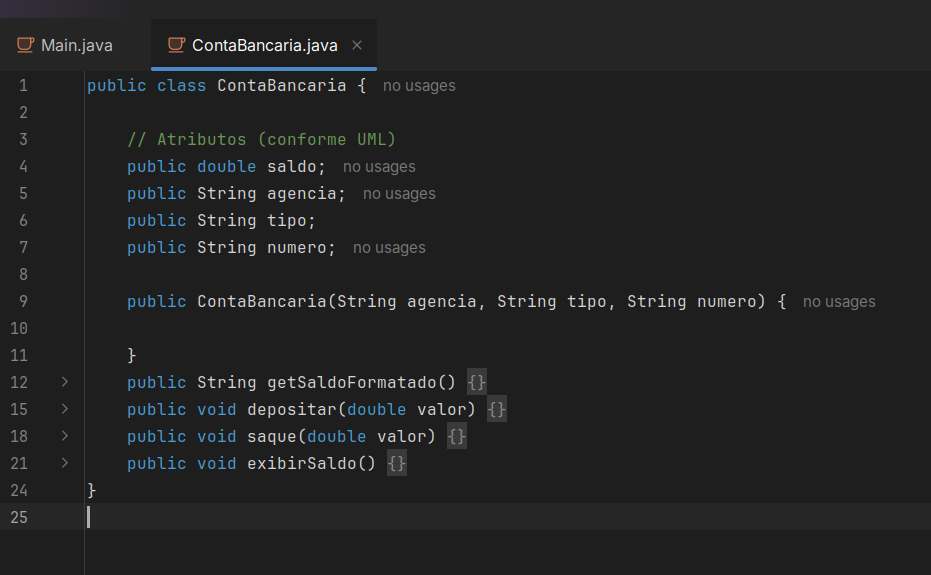
\includegraphics[width=\linewidth]{classeContaCodigo.png}
    % \caption{Representação ilustrativa de uma classe em JAVA}
\end{figure}
\end{frame}
\section{Atributos de uma classe}

\begin{frame}{Atributos na Classe ContaBancaria}

\begin{block}{Definição no Contexto da Classe}
Atributos são variáveis declaradas dentro de uma classe que
vão representar o \textbf{estado} dos objetos criados a partir dela. Na classe \texttt{ContaBancaria}, os atributos representam
as informações que caracterizam cada conta criada no sistema.
\end{block}

\begin{block}{Função dos Atributos}
Eles armazenam o \textbf{estado da conta}, ou seja:
\begin{itemize}
    \item Quanto dinheiro ela possui
    \item A qual agência pertence
    \item Qual o seu tipo
    \item Qual o seu número identificador
\end{itemize}
\end{block}

\begin{block}{Importante}
Cada objeto criado a partir da classe \texttt{ContaBancaria}
possui seus próprios valores para esses atributos,
garantindo independência entre as contas.
\end{block}

\end{frame}
\begin{frame}{Estrutura dos Atributos da ContaBancaria}

\begin{block}{Declaração na Classe}
\begin{itemize}
    \item \texttt{public double saldo;}
    \item \texttt{public String agencia;}
    \item \texttt{public String tipo;}
    \item \texttt{public String numero;}
\end{itemize}
\end{block}
 

\begin{block}{Análise Técnica}
\begin{itemize}
    \item \textbf{saldo \(double\)}: armazena valores numéricos com casas decimais.
    \item \textbf{agencia \(String\)}: identifica a unidade bancária.
    \item \textbf{tipo \(String\)}: classifica a conta (corrente, poupança).
    \item \textbf{numero \(String\)}: identifica unicamente a conta.
\end{itemize}
\end{block}

\begin{block}{Interpretação}
Esses atributos definem o \textbf{estado interno}
de cada instância da classe.
\end{block}

\end{frame}
\begin{frame}{Atributos de diferentes classes}

\begin{figure}
    \centering
    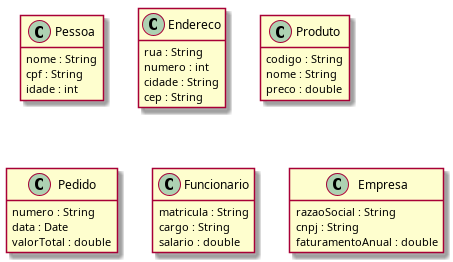
\includegraphics[width=\linewidth]{atributos.png}
    % \caption{Representação ilustrativa de uma classe em JAVA}
\end{figure}
\end{frame}
\section{Métodos}

\begin{frame}{Métodos em Orientação a Objetos}
 \begin{figure}
    \centering
    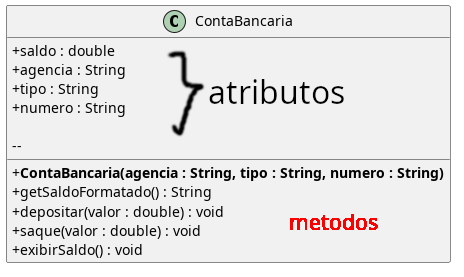
\includegraphics[width=0.6\linewidth]{ContaBancariaUml.png}
    \caption{Representação ilustrativa de uma classe em UML}
\end{figure}
\begin{block}{Definição}
  
Métodos são funções definidas dentro de uma classe
que representam o \textbf{comportamento} dos objetos.
\end{block}
\end{frame}

\begin{frame}{Métodos em Orientação a Objetos}

\begin{block}{Função dos Métodos}
\begin{itemize}
    \item Manipular os atributos (estado)
    \item Executar operações relacionadas ao objeto
    \item Definir o que o objeto é capaz de fazer
\end{itemize}
\end{block}

\begin{block}{Estrutura Geral}
\texttt{modificador retorno nomeMetodo(parametros)}

Exemplo:
\texttt{public void depositar(double valor)}
\end{block}
 \begin{figure}
    \centering
    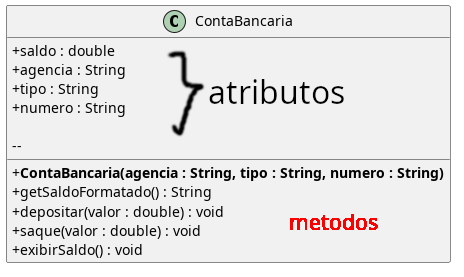
\includegraphics[width=0.6\linewidth]{ContaBancariaUml.png}
    \caption{Representação ilustrativa de uma classe em UML}
\end{figure}
\end{frame}
\begin{frame}{Métodos da Classe ContaBancaria}

\begin{block}{Construtor}
\texttt{ContaBancaria(String agencia, String tipo, String numero)}
\end{block}

\begin{block}{Métodos Declarados}
\begin{itemize}
    \item \texttt{getSaldoFormatado() : String}
    \item \texttt{depositar(double valor) : void}
    \item \texttt{saque(double valor) : void}
    \item \texttt{exibirSaldo() : void}
\end{itemize}
\end{block}

\begin{block}{Observação}
Esses métodos definem as operações que podem ser realizadas
sobre uma conta bancária.
\end{block}

\end{frame}
\begin{frame}{Explicação dos Métodos da ContaBancaria}

\begin{block}{getSaldoFormatado()}
Retorna o valor do saldo convertido para uma
representação textual formatada (moeda).
\end{block}

\begin{block}{depositar(double valor)}
Adiciona um valor ao atributo \texttt{saldo},
alterando o estado interno da conta.
\end{block}

\begin{block}{saque(double valor)}
Subtrai um valor do \texttt{saldo},
caso haja saldo suficiente.
\end{block}

\begin{block}{exibirSaldo()}
Apresenta ao usuário o saldo atual da conta.
\end{block}

\end{frame}

\begin{frame}{Métodos em diferentes classes}

\begin{figure}
    \centering
    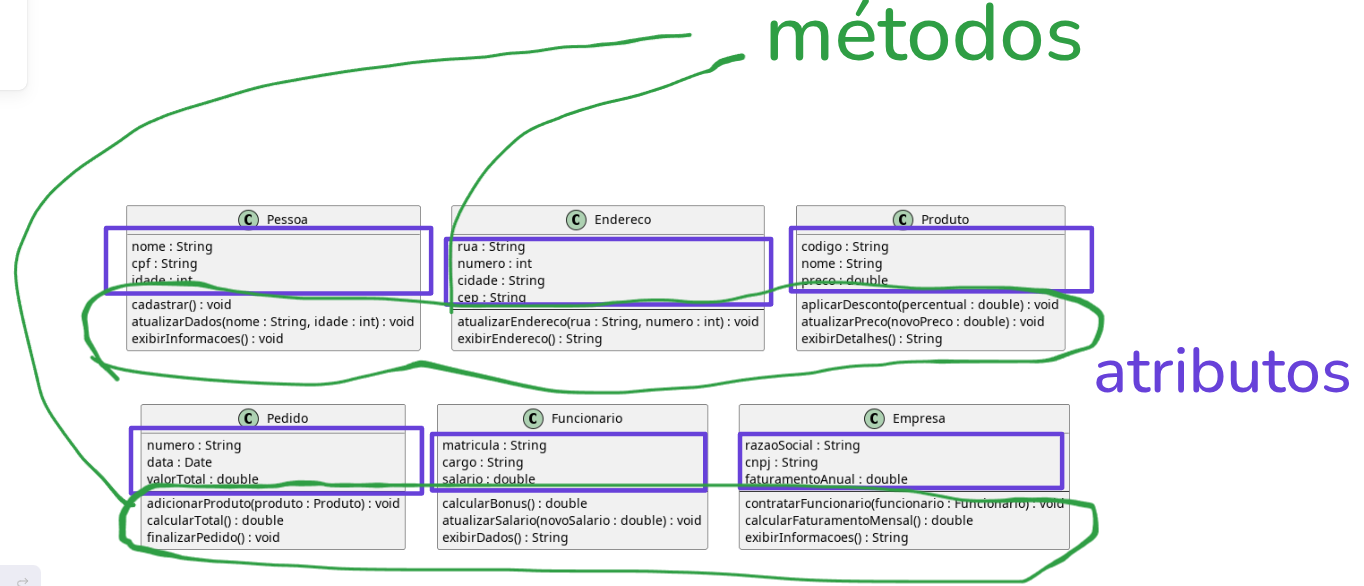
\includegraphics[width=\linewidth]{metodos.png}
    % \caption{Representação ilustrativa de uma classe em JAVA}
\end{figure}
\end{frame}

\section{Método Construtor}
\begin{frame}[fragile]{Método Construtor}

\begin{block}{Definição}
O \textbf{método construtor} é um método especial de uma classe responsável por
\textbf{inicializar os atributos do objeto no momento de sua criação}.
\end{block}

\begin{block}{Características}
\begin{itemize}
    \item Possui o \textbf{mesmo nome da classe}.
    \item É executado automaticamente quando o objeto é instanciado.
    \item Normalmente define o estado inicial dos atributos.
    \item Pode receber parâmetros.
\end{itemize}
\end{block}
 
\begin{block}{Exemplo Geral em Java}
\begin{verbatim}
public class Pessoa {
    private String nome;

    public Pessoa(String nome) {
        this.nome = nome;
    }
}
\end{verbatim}
\end{block}

\end{frame}
\begin{frame}[fragile]{Método Construtor na Classe ContaBancaria}

\begin{verbatim}
public class ContaBancaria {

    private String titular;
    private int numero;
    private double saldo;

    public ContaBancaria(String titular, int numero) {
        this.titular = titular;
        this.numero = numero;
        this.saldo = 0.0;
    }
}
\end{verbatim}

\begin{block}{Identificação}
\begin{itemize}
    \item O método ContaBancaria(...) é o construtor
    \item Nome idêntico ao da classe
    \item Inicializa os atributos
\end{itemize}
\end{block}

\end{frame}
\section{Posicionamento no código JAVA}

\begin{frame}{Posicionamento no código JAVA}

\begin{figure}
    \centering
    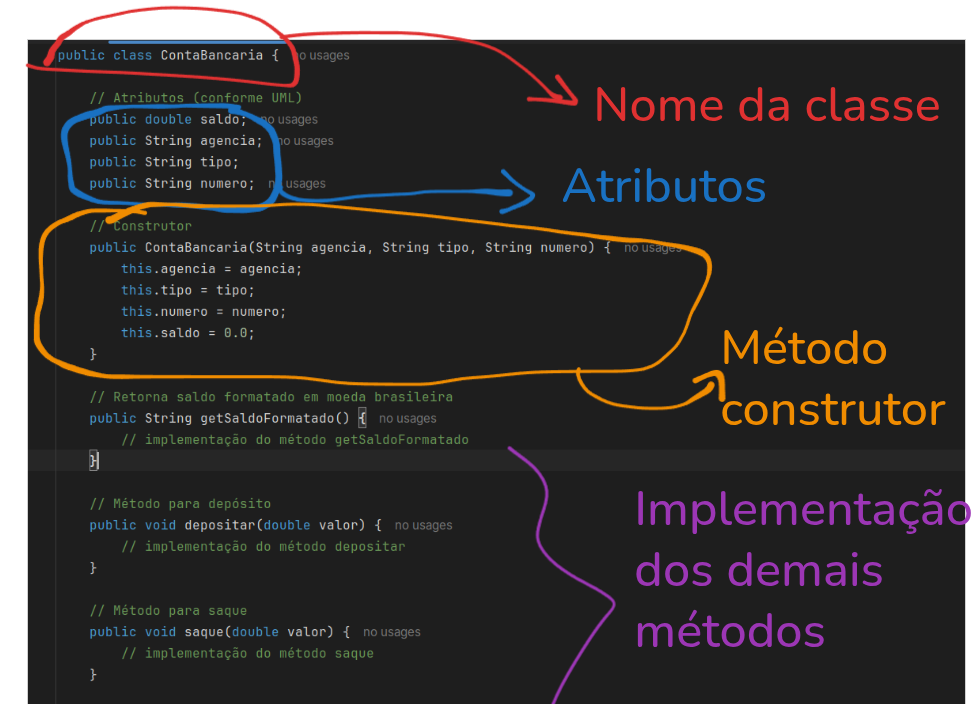
\includegraphics[width=\linewidth]{posicionamento.png}
    % \caption{Representação ilustrativa de uma classe em JAVA}
\end{figure}
\end{frame}

\begin{frame}{Código completo com explicação: parte 1}
 \begin{figure}
    \centering
    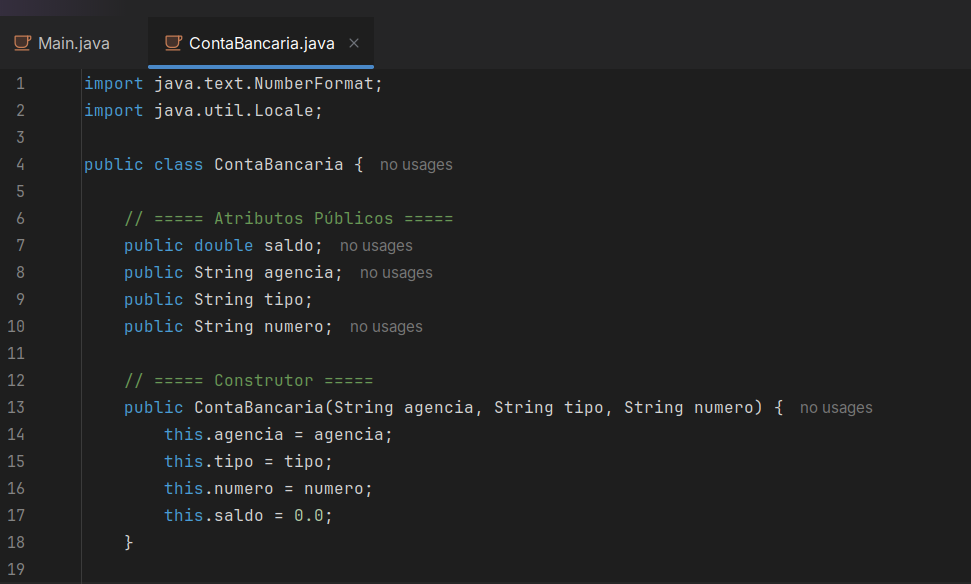
\includegraphics[width=0.8\linewidth]{implementacao1.png}
\end{figure}
\begin{block}{Definição}
    No início do código há a importação de códigos de terceiros com \texttt{import java.text.NumberFormat;} e \texttt{import java.util.Locale;}, que são bibliotecas para formatação de números e localização. Depois vem a declaração da classe \texttt{ContaBancaria} e a definição de seus atributos, seguido do método construtor. 


\end{block}
\end{frame}
\section{Código completo com explicação}

\begin{frame}{Código completo com explicação: parte 1}
 \begin{figure}
    \centering
    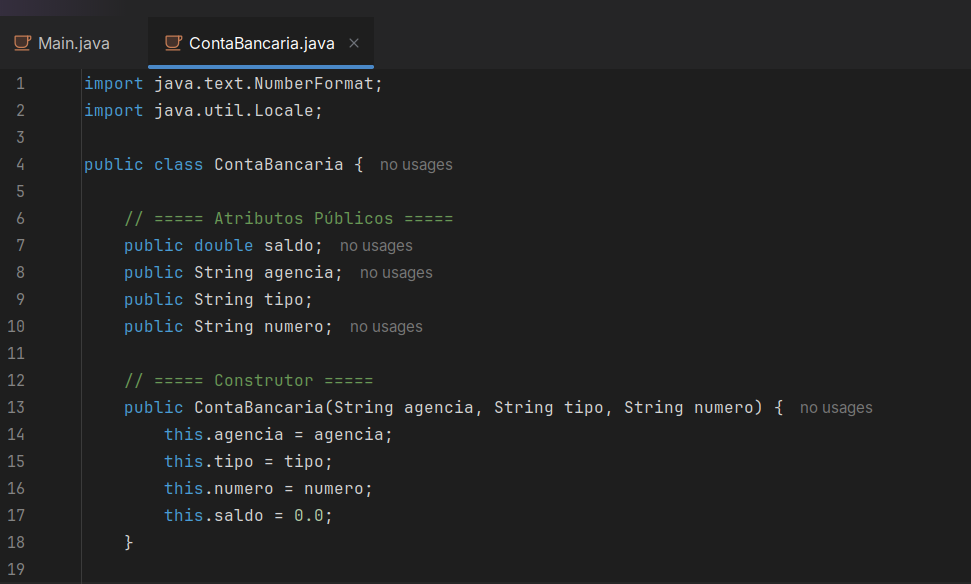
\includegraphics[width=0.8\linewidth]{implementacao1.png}
\end{figure}
\begin{block}{Definição}
    Observe que o método construtor tem o mesmo nome da classe e é responsável por inicializar os atributos \texttt{agencia}, \texttt{tipo} e \texttt{numero} com os valores passados como parâmetros, além de definir o saldo inicial como zero. Isso é interessante a fim de garantir que toda conta criada tenha um estado inicial consistente.
\end{block}
\end{frame}

\begin{frame}{Código completo com explicação: parte 2}
 \begin{figure}
    \centering
    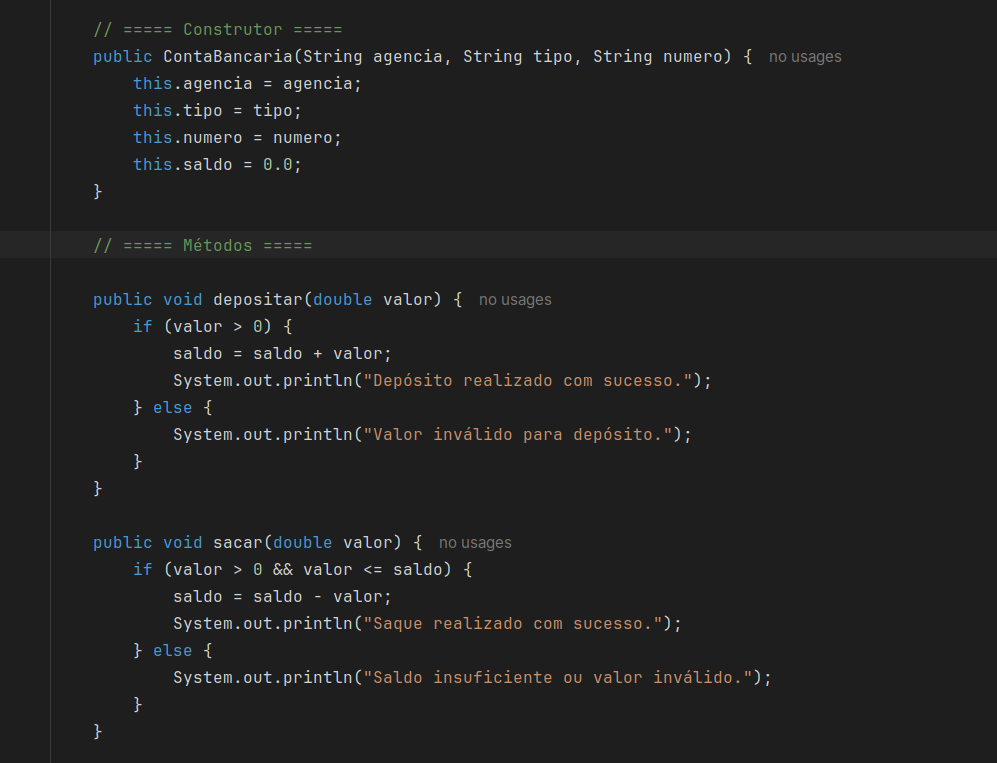
\includegraphics[width=0.6\linewidth]{implementacao2.png}
\end{figure}
\begin{block}{Definição}
    Logo abaixo há a implementação dos demais métodos da classe, como \texttt{getSaldoFormatado()}, que utiliza a biblioteca \texttt{NumberFormat} para formatar o saldo como moeda, e os métodos \texttt{depositar}, \texttt{saque} e \texttt{exibirSaldo}, que manipulam o estado da conta e apresentam informações ao usuário.
\end{block}
\end{frame}
\begin{frame}{Código completo com explicação: parte 3}
 \begin{figure}
    \centering
    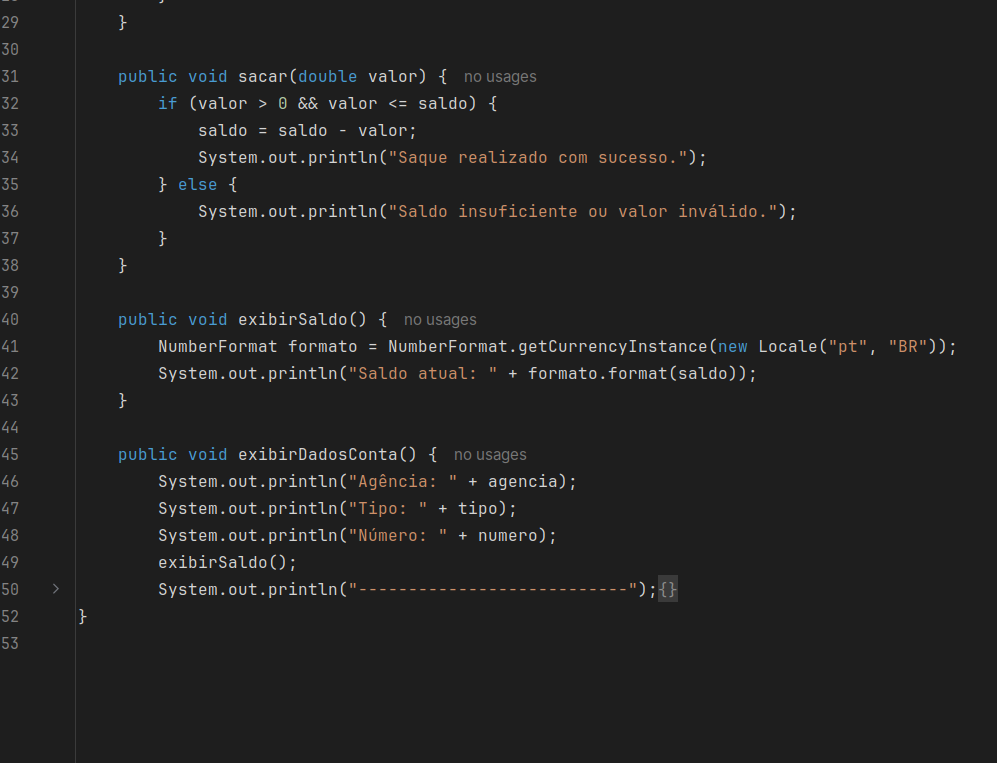
\includegraphics[width=0.6\linewidth]{implementacao3.png}
\end{figure}
\begin{block}{Definição}
    Logo abaixo há a implementação dos demais métodos da classe, como \texttt{getSaldoFormatado()}, que utiliza a biblioteca \texttt{NumberFormat} para formatar o saldo como moeda, e os métodos \texttt{depositar}, \texttt{saque} e \texttt{exibirSaldo}, que manipulam o estado da conta e apresentam informações ao usuário.
\end{block}
\end{frame}
\begin{frame}{Código completo com explicação: parte 4 (FINAL)}
 \begin{figure}
    \centering
    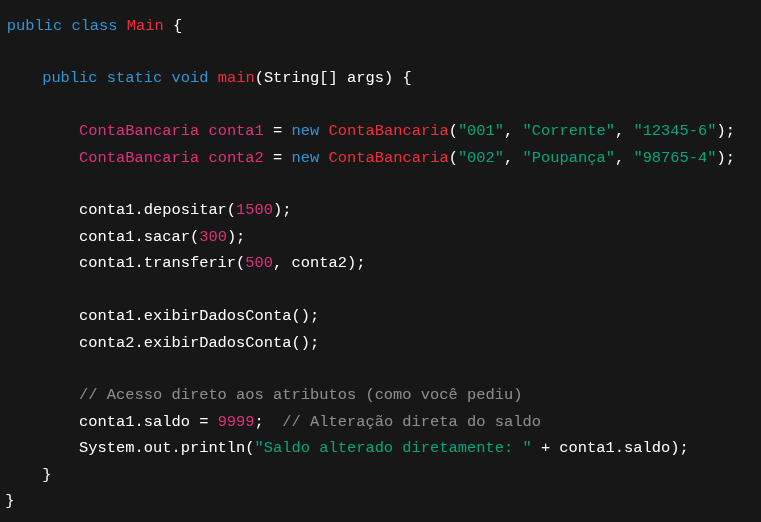
\includegraphics[width=0.7\linewidth]{criacaoObjetos.png}
\end{figure}
\begin{block}{Definição}
    Aqui temos a criação de duas instâncias da classe \texttt{ContaBancaria}, representando duas contas bancárias distintas. Cada conta tem seus próprios valores para os atributos, demonstrando a independência entre os objetos criados a partir da mesma classe.
\end{block}
\end{frame}
\end{document}
